%% Lecture 29

\section{Krylov Methods}

Krylov methods are iterative methods to solve a linear system $A\vec{x}=\vec{b}$. They are different from fixed-point methods such as Jacobi. Given a vector $\vec{d}\in \mathbb{R}^n$, the $m$\textsuperscript{th} Krylov space is

\begin{equation*}
    \mathcal{K}_m (A, \vec{d}) = \text{span}\{ \vec{d}, A\vec{d}, A^2 \vec{d}, \ldots, A^{m-1}\vec{d}\}
\end{equation*}

At the $m$\textsuperscript{th} iterate of a Krylov method, it seeks the best solution to $A\vec{x}=\vec{b}$ in $\mathcal{K}_m(A, \vec{d})$. Since $\mathcal{K}_m \subseteq \mathcal{K}_{m+1}$, the error always decreases with $m$. The two main Krylov methods that we'll consider:

\begin{enumerate}[1)]
    \item Conjugate Gradient(CG)
    \item Generalized Minimal Residual method (GMRES)
\end{enumerate}

Varients of these methods are preconditioned versions (pCG, pGMRES), Biconjugate Gradient method (BiCG), and Biconjugate Gradient Stabilized method (BiCGSTAB).

We will begin our discussion of Krylov methods by exploring the Conjugate Gradient method. Much of these notes come from the paper by \cite{shewchuk-1994} , where a deeper analysis is provided.

\subsection{Making $A\vec{x}=\vec{b}$ a Minimization Problem}

Suppose $A$ is symmetric ($A=A^T$) and positive definite:

\begin{equation*}
    \vec{x}^{\,T}A\vec{x} > 0 \qquad \forall \vec{x}\neq\vec{0}
\end{equation*}

These matrices are typical in many problems including finite difference and finite element methods. Given such a matrix, it is gauranteed to be invertible.

Given the linear system $A\vec{x} = \vec{b}$, we define the quadratic form (function)

\begin{align*}
    &f(\vec{x}) = \frac{1}{2}\vec{x}^{\,T}A\vec{x} - \vec{b}^{\,T}\vec{x} \\
    &f: \mathbb{R}^n \rightarrow \mathbb{R}
\end{align*}
Because $A$ is positive definite, the function $f$ is shaped like an $n$-dimensional parabaloid (ie.\ a bowl). Therefore it has a single minimum.

\begin{equation*}
    \nabla f =
    \begin{bmatrix}
        \partial f / \partial x_1\\
        \vdots \\
        \partial f / \partial x_n\\
    \end{bmatrix}
    =\vec{0}
\end{equation*}

We have that

\begin{align*}
    f(\vec{x}) = f(x_1, x_2, \ldots, x_n) &= \frac{1}{2} \sum_{i=1}^{n} x_i \sum_{j=1}^{n} a_{ij} x_j - \sum_{i=1}^{n} b_i x_i \\
    \Rightarrow \frac{\partial f}{\partial x_k} &=\frac{1}{2} \sum_{j=1}^{n} a_{kj} x_j + \frac{1}{2} \sum_{i=1}^{n} x_i a_{ik} - b_k \\
    &=\frac{1}{2} \sum_{j=1}^{n} a_{kj} x_j + \frac{1}{2} \sum_{i=1}^{n} a_{ik} x_i - b_k \\
    &= \frac{1}{2} (A\vec{x})_k + \frac{1}{2} (A^T\vec{x})_k - b_k \\
    \Rightarrow \nabla f &= \frac{1}{2} A\vec{x} + \frac{1}{2} A^T\vec{x} - \vec{b} \\
    &= \frac{1}{2} A\vec{x} + \frac{1}{2} A\vec{x} - \vec{b} \\
    &= A\vec{x} - \vec{b} \\
    \Rightarrow \nabla f &= 0 \Leftrightarrow A\vec{x} - \vec{b} = 0
    \Leftrightarrow A \vec{x} = \vec{b}
\end{align*}
That is, the solution of $A \vec{x} = \vec{b}$ is at the (local) minimum of $f$. Therefore, if we can minimize $f$, we have solved $A \vec{x} = \vec{b}$.


\subsection{Method of Steepest Decent and Line Search}
Imagine you are in a high-dimensional bowl and your goal is to reach the bottom as fast as possible. Moreover, you can not see the bottom and can only see what is happening in a small region around you.

At each step (iteration), we have 2 choices

\begin{enumerate}[1)]
    \item Which direction to go?
    \item How far should you go in that direction?
\end{enumerate}

A natural choice for the direction is the direction of steepest descent. For any function $f$, the method of steepest descent is $\pm \nabla f$. In our case, the steepest decent is in the direction $-\nabla f$. We already know that

\begin{equation*}
    -\nabla f = \vec{b} - A \vec{x}
\end{equation*}

%% Lecture 30


Therefore, given a current iterate $\vec{x}^{\,(i)}$, the new iterate should be

\begin{equation*}
    \vec{x}^{\,(i+1)} = \vec{x}^{\,(i)} + \alpha^{(i)}\vec{r}^{\,(i)}
\end{equation*}
where $\vec{r}^{\,(i)} = \vec{b} - A\vec{x}^{\,(i)}$ is the residual, and $\alpha^{(i)}\in\mathbb{R}^{+}$ is the step size. To find the optimal $\alpha^{(i)}$, we optimize $f\left(\vec{x}^{\,(i+1)}\right)$. This is a line search and the role of $\alpha^{(i)}$. If $n=2$, we can draw that is happening

\begin{center}
    
    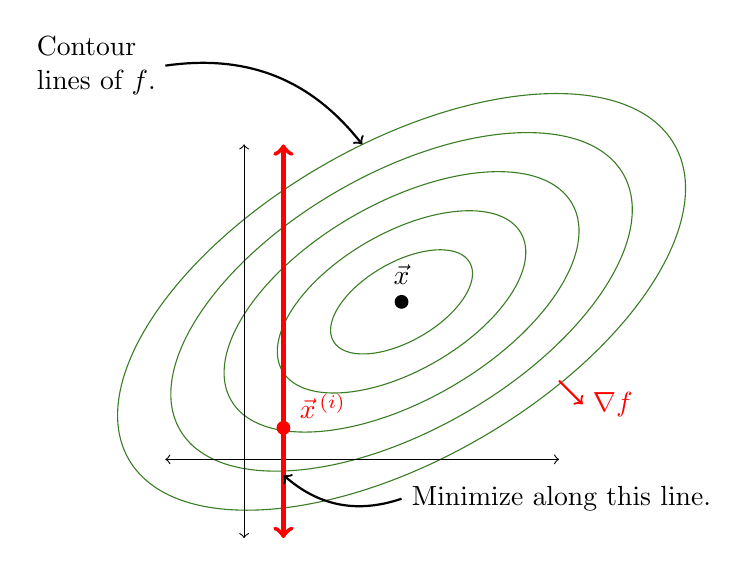
\begin{tikzpicture}
        \foreach \size in {1, 1.75, ..., 4} {
            \draw[OliveGreen, scale=\size, rotate=30] (0,0) ellipse (1cm and .5cm);
        };
        \node[circle, inner sep=0, minimum size=5pt,fill, label={$\vec{x}$}]() at (0,0){};

        \draw[<->] (-2, -3) -- (-2, 2);
        \draw[<->] (-3, -2) -- (2, -2);

        \node[ red, circle, inner sep=0, minimum size=5pt, fill,
        label={[red, xshift=5mm, yshift=-1mm]$\vec{x}^{\,(i)}$}
        ] () at (-1.5, -1.6){};

        \draw[<->, red, ultra thick] (-1.5, -3) -- (-1.5, 2);

        \draw[<-, thick] (-1.5, -2.2) to[bend right=30] (0, -2.5) node[right] () {Minimize along this line.};

        \draw[<-, thick] (-.5, 2) to[bend right=30] (-3, 3) node[left, xshift=5mm, text width=2cm] () {Contour lines of $f$.};

        \draw[->, thick, red] (2, -1) -- (2.3, -1.3) node[right](){$\nabla f$};
    \end{tikzpicture}

\end{center}

To find the optimal $\alpha^{(i)}$, we optimize

\begin{equation*}
    f\left(\vec{x}^{\,(i+1)}\right) = f\left(\vec{x}^{\,(i)} + \alpha\vec{r}^{\,(i)}\right)
\end{equation*}
with respect to $\alpha$. This can be done by solving

\begin{align*}
    \frac{d}{d\alpha}f\left(\vec{x}^{\,(i+1)}\right) &= 0\\
    \Rightarrow \frac{d}{d\alpha}f\left(\vec{x}^{\,(i)} + \alpha\vec{r}^{\,(i)}\right) &= 0\\
\end{align*}

\underline{Claim:}
\begin{equation*}
         \frac{d}{d\alpha}f\left(\vec{x}^{\,(i)} + \alpha\vec{r}^{\,(i)}\right) = \nabla f\left(\vec{x}^{\,(i)} + \alpha\vec{r}^{\,(i)}\right)\cdot \vec{r}^{\,(i)}
\end{equation*}

\underline{Proof:}
\begin{align*}
    &\frac{d}{d\alpha}f\left(\vec{x}^{\,(i)} + \alpha\vec{r}^{\,(i)}\right) =
    \frac{d}{d\alpha}f\left(
    \begin{bmatrix}
        x^{(i)}_1 + \alpha r^{(i)}_1 \\
        x^{(i)}_2 + \alpha r^{(i)}_2 \\
        \vdots \\
        x^{(i)}_n + \alpha r^{(i)}_n \\
    \end{bmatrix}
    \right)\\
    = &\frac{\partial f}{\partial x_1}\bigg\rvert_{\vec{x}^{\,(i)} + \alpha\vec{r}^{\,(i)}} r_{(1)}^{(i)}
    + \frac{\partial f}{\partial x_2}\bigg\rvert_{\vec{x}^{\,(i)} + \alpha\vec{r}^{\,(i)}} r_{(2)}^{(i)}\\
    & + \ldots + \frac{\partial f}{\partial x_n}\bigg\rvert_{\vec{x}^{\,(i)} + \alpha\vec{r}^{\,(i)}} r_{(n)}^{(i)}\\
    &= \nabla f\left(\vec{x}^{\,(i)} + \alpha\vec{r}^{\,(i)}\right)\cdot \vec{r}^{\,(i)}
\end{align*}


Therefore, the optimal $\alpha^{(i)}$ satisfies

\begin{equation*}
    \nabla f\left(\vec{x}^{\,(i)} + \alpha \vec{r}^{\,(i)}\right)\cdot \vec{r}^{\,(i)} = 0
\end{equation*}

That is, $\alpha^{(i)}$ should be chosen to that $\vec{r}^{\,(i)}$ is orthogonal to $\nabla f\left(\vec{x}^{\,(i+1)}\right)$

\begin{center}
    
    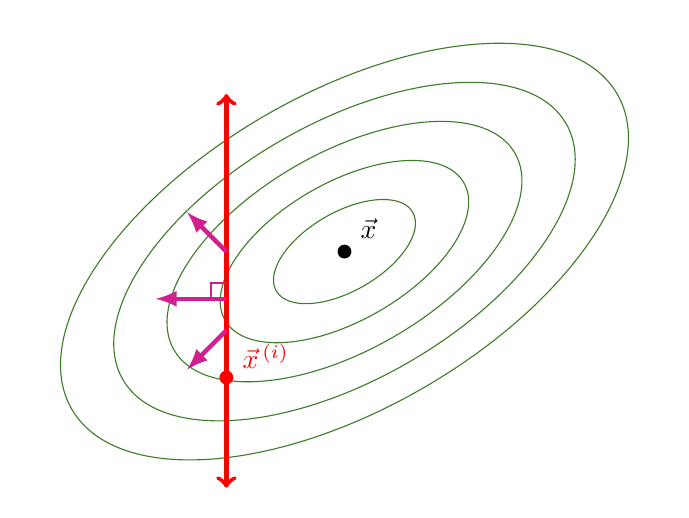
\begin{tikzpicture}
        \foreach \size in {1, 1.75, ..., 4} {
            \draw[OliveGreen, scale=\size, rotate=30] (0,0) ellipse (1cm and .5cm);
        };
        \node[circle, inner sep=0, minimum size=5pt,fill, label={30:$\vec{x}$}]() at (0,0){};


        \node[ red, circle, inner sep=0, minimum size=5pt, fill,
        label={[red, xshift=5mm, yshift=-1mm]$\vec{x}^{\,(i)}$}
        ] () at (-1.5, -1.6){};

        \draw[<->, red, ultra thick] (-1.5, -3) -- (-1.5, 2);

        \draw[->,>=latex, VioletRed, ultra thick] (-1.5, -.6) -- (-2.4, -.6);
        \draw[->,>=latex, VioletRed, ultra thick] (-1.5, -1) -- (-2, -1.5);
        \draw[->,>=latex, VioletRed, ultra thick] (-1.5, 0) -- (-2, .5);
        \draw[VioletRed, thick] (-1.7, -.6) |- (-1.5, -.4);
    \end{tikzpicture}

\end{center}

To find this value of $\alpha$, since $\nabla f\left(\vec{x}^{\,(i+1)}\right)=-\vec{r}^{\,(i+1)}$, we need $\vec{r}^{\,(i+1)} \cdot \vec{r}^{\,(i)}=0$

\begin{align*}
    &\Leftrightarrow \vec{r}^{\,(i+1)T}  \vec{r}^{\,(i)}=0\\
    &\Leftrightarrow \left(\vec{b} - A\vec{x}^{\,(i+1)}\right)^T \vec{r}^{\,(i)}=0\\
    &\Leftrightarrow \left(\vec{b} - A\left(\vec{x}^{\,(i)} + \alpha \vec{r}^{\,(i)}\right)\right)^T \vec{r}^{\,(i)}=0\\
    &\Leftrightarrow
    \left(\vec{b} - A\vec{x}^{\,(i)}\right)^T
    \vec{r}^{\,(i)}
    - \alpha \left( A\vec{r}^{\,(i)}\right)^T
    \vec{r}^{\,(i)}
    =0\\
    &\Leftrightarrow
    \vec{r}^{\,(i)T}
    \vec{r}^{\,(i)}
    - \alpha \vec{r}^{\,(i)T} A^T
    \vec{r}^{\,(i)}
    = 0 \\
    &\Leftrightarrow
    \vec{r}^{\,(i)T}
    \vec{r}^{\,(i)}
    - \alpha \vec{r}^{\,(i)T} A
    \vec{r}^{\,(i)}
    = 0 \\
    &\Leftrightarrow \alpha = \frac{\vec{r}^{\,(i)T}\vec{r}^{\,(i)}}{\vec{r}^{\,(i)T}A\vec{r}^{\,(i)}}
\end{align*}


Therefore the optimal $\alpha$ to take in the line search is
\begin{equation*}
    \alpha^{(i)} = \frac{\vec{r}^{\,(i)T}\vec{r}^{\,(i)}}{\vec{r}^{\,(i)T}A\vec{r}^{\,(i)}}
\end{equation*}

Therefore, our algorithm to solve $A\vec{x}=\vec{b}$ is


\begin{algorithmic}
    \FOR{$i=0, 1, 2, \ldots$}
    \STATE $\vec{r}^{\,(i)} = \vec{b} - A\vec{x}^{\,(i)}$
    \STATE $    \alpha^{(i)} = \frac{\vec{r}^{\,(i)T}\vec{r}^{\,(i)}}{\vec{r}^{\,(i)T}A\vec{r}^{\,(i)}} $
    \STATE $\vec{x}^{\,(i+1)} = \vec{x}^{\,(i)} + \alpha^{(i)}\vec{r}^{\,(i)}$
    \ENDFOR
\end{algorithmic}

By choosing the optimal $\alpha^{(i)}$, we have that consecutive search directions are orthogonal. This creates a zigzag pattern as $\vec{x}^{\,(i)}$ converges to $\vec{x}$.


\begin{center}
    
    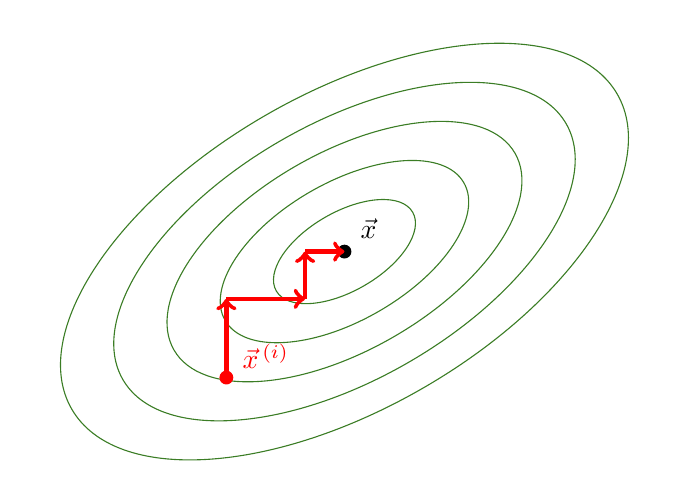
\begin{tikzpicture}
        \foreach \size in {1, 1.75, ..., 4} {
            \draw[OliveGreen, scale=\size, rotate=30] (0,0) ellipse (1cm and .5cm);
        };
        \node[circle, inner sep=0, minimum size=5pt,fill, label={30:$\vec{x}$}]() at (0,0){};

        \node[ red, circle, inner sep=0, minimum size=5pt, fill,
        label={[red, xshift=5mm, yshift=-1mm]$\vec{x}^{\,(i)}$}
        ] () at (-1.5, -1.6){};

        \draw[->, red, ultra thick] (-1.5, -1.6) -- (-1.5, -.6);
        \draw[->, red, ultra thick] (-1.5, -0.6) -- (-0.5, -0.6);
        \draw[->, red, ultra thick] (-0.5, -0.6) -- (-0.5, 0);
        \draw[->, red, ultra thick] (-0.5, 0) -- (0, 0);

    \end{tikzpicture}

\end{center}



We define the error at iteration $i$ to be

\begin{equation*}
    \vec{e}^{\,(i)} =\vec{x}^{\,(i)} - \vec{x}
\end{equation*}
To analyze the convergence of steepest descent, it is convenient to use the energy norm

\begin{equation*}
    \lvert\lvert \vec{e}\, \rvert\rvert_A :=\sqrt{\vec{e}^{\,T}A\vec{e}}
\end{equation*}

Since A is spd, all its eigenvalues are real and positive, and are also the singular values of $A$. Letting $\lambda_{\max}$ and $\lambda_{\min}$ be the biggest and smallest eigenvalues, then

\begin{equation*}
    \lvert\lvert \vec{e}^{\,(i+1)} \rvert\rvert_A
    =\lvert\lvert \vec{e}^{\,(i)} \rvert\rvert_A\omega
\end{equation*}
where
\begin{equation*}
    \omega \leq \frac{\kappa - 1}{\kappa+1}
\end{equation*}
where $\kappa = \lambda_{\max}/\lambda_{\min} \geq 1$ is the condition number of $A$. Therefore, convergence is fastest when $\kappa\approx 1$.


%% Lecture 31

In general, we have

\begin{align*}
    || \vec{e}^{\,(i)} ||_A &= || \vec{e}^{\,(i-1)} ||_A\omega = || \vec{e}^{\,(i-2)} ||_A\omega^2\\
    &= || \vec{e}^{\,(0)} ||_A \left(\frac{\kappa-1}{\kappa+1}\right)^i
\end{align*}

\subsection{A better choice for the search direction}

Steepest descent has a major issue. The search direction at differenet iterations are often very similar. It would be nice if we went exactly the correct amount in that direction so that we find the solution by the $n$\textsuperscript{th} iterate.


\begin{center}
    
    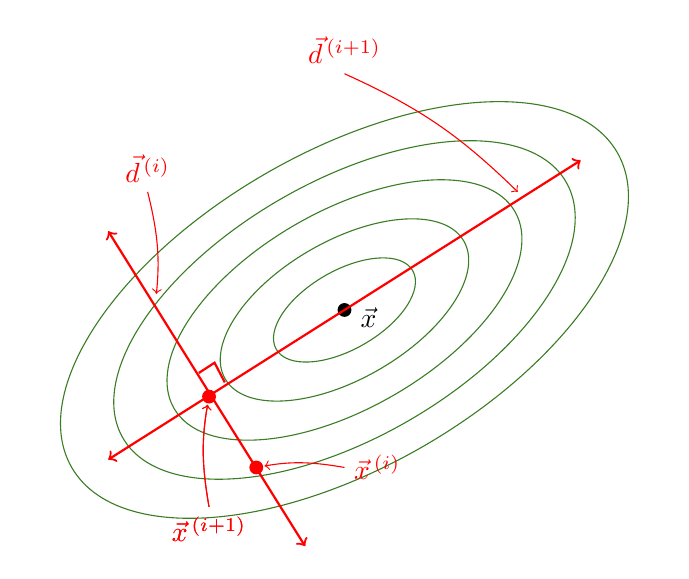
\begin{tikzpicture}
        \foreach \size in {1, 1.75, ..., 4} {
            \draw[OliveGreen, scale=\size, rotate=30] (0,0) ellipse (1cm and .5cm);
        };
        % \node[circle, inner sep=0, minimum size=5pt,fill, label={30:$\vec{x}$}]() at (0,0){};
        \node[circle, inner sep=0, minimum size=5pt,fill, label={[yshift=2mm]-30:$\vec{x}$}]() at (0,0){};

        \draw[<->, thick, red] (3, 1.9) -- (-3, -1.9);
        \draw[<->, thick, red] (-3, 1) -- (-.5, -3);

        \node[red, circle, inner sep=0, minimum size=5pt,fill] () at (-1.12, -2){};
        \node[red, circle, inner sep=0, minimum size=5pt,fill] () at (-1.72, -1.1){};
        \draw[thick, red] (-1.85, -0.8) -- (-1.65, -0.67) -- (-1.52, -0.92);

        \draw[<-, shorten <=3pt, red] (-1.12, -2) to[bend left=10] (0, -2) node[right] () {$\vec{x}^{\,(i)}$};
        \draw[<-, shorten <=3pt, red] (-1.72, -1.1) to[bend right=10] (-1.72, -2.5) node[below] () {$\vec{x}^{\,(i+1)}$};
        \draw[<-, shorten <=3pt, red] (-1.72, -1.1) to[bend right=10] (-1.72, -2.5) node[below] () {$\vec{x}^{\,(i+1)}$};
        \draw[<-, shorten <=3pt, red] (-2.4, .1) to[bend right=10] (-2.5, 1.5) node[above] () {$\vec{d}^{\,(i)}$};
        \draw[<-, red] (2.2, 1.5) to[bend right=10] (0, 3) node[above] () {$\vec{d}^{\,(i+1)}$};

    \end{tikzpicture}

\end{center}


Instead of looking in the steepest descent direction, we will search in new directions

\begin{equation*}
    \vec{d}^{\,(0)}, \vec{d}^{\,(1)}, \ldots, \vec{d}^{\,(n-1)}
\end{equation*}
where the search directions are mutually orthogonal. Then each iteration will be

\begin{equation*}
    \vec{x}^{\,(i+1)} = \vec{x}^{\,(i)}+ \alpha^{(i)}\vec{d}^{\,(i)}
\end{equation*}
Since we require $\vec{x}^{\,(i+1)}$ to be exact in the direction $\vec{d}^{\,(i)}$, the error $\vec{e}^{\,(i+1)} = \vec{x}^{\,(i+1)}-\vec{x}$ needs to be orthogonal to $\vec{d}^{\,(i+1)}$. Since

\begin{align*}
    \vec{x}^{\,(i+1)} &= \vec{x}^{\,(i)}+ \alpha^{(i)}\vec{d}^{\,(i)} \\
    \vec{x}^{\,(i+1)} -\vec{x} &= \vec{x}^{\,(i)}- \vec{x}+ \alpha^{(i)}\vec{d}^{\,(i)}  \\
    \vec{e}^{\,(i+1)} &= \vec{e}^{\,(i)}+ \alpha^{(i)}\vec{d}^{\,(i)} \\
\end{align*}
Therefore
\begin{align*}
    \vec{d}^{\,(i)T}\vec{e}^{\,(i+1)} &= 0 \\
    \vec{d}^{\,(i)T}(\vec{e}^{\,(i)}+ \alpha^{(i)}\vec{d}^{\,(i)}) &= 0 \\
    \alpha^{(i)} = - \frac{\vec{d}^{\,(i)T}\vec{e}^{\,(i)}}{\vec{d}^{\,(i)T}\vec{d}^{\,(i)}}
\end{align*}

Unfortunately, we don't know what the error, $\vec{e}^{\,(i)}$, is. The solution is to not choose orthogonal search directions $\vec{d}^{\,(i)}$. Instead we use search directions that are $A$-orthogonal. That is
\begin{equation*}
    \vec{d}^{\,(i)T}A\vec{d}^{\,(i)} = 0 \qquad \forall i\neq j
\end{equation*}
Then instead of requireing $\vec{e}^{\,(i+1)}$ to be orthogonal to $\vec{d}^{\,(i)}$, we require that $\vec{e}^{\,(i+1)}$ is $A$-orthogonal to $\vec{d}^{\,(i)}$. This is indeed a good choice since

\begin{align*}
    &\frac{d}{d\alpha} f\left(\vec{x}^{\,(i+1)}\right) = 0 \\
    &\Leftrightarrow \nabla f\left(\vec{x}^{\,(i+1)}\right)^T \frac{d}{d\alpha}\vec{x}^{\,(i+1)} =0 \\
    &\Leftrightarrow -\vec{r}^{\,(i+1)T}\vec{d}^{\,(i)} = 0 \\
    &\Leftrightarrow -\vec{d}^{\,(i)T} \vec{r}^{\,(i+1)}= 0 \\
    &\Leftrightarrow -\vec{d}^{\,(i)T} A\vec{e}^{\,(i+1)}= 0 \\
\end{align*}

Since $A\vec{e}^{\,(i+1)} = A\left(\vec{x}^{\,(i+1)} -\vec{x}\right)=A\vec{x}^{\,(i+1)} - \vec{b} = -\vec{r}^{\,(i+1)}$

That is, if $\vec{e}^{\,(i+1)}$ is $A$-orthogonal to $\vec{d}^{\,(i)}$, then $\vec{x}^{\,(i+1)} = \vec{x}^{\,(i)} + \alpha^{(i)}\vec{d}^{\,(i)}$ minimizes $f$ along this line search direction. To find $\alpha^{(i)}$, we require
\begin{align*}
    \vec{d}^{\,(i)T}A\vec{e}^{\,(i+1)} &= 0 \\
    \Rightarrow\vec{d}^{\,(i)T}A(\vec{e}^{\,(i)}+ \alpha^{(i)}\vec{d}^{\,(i)}) &= 0 \\
    \Rightarrow\alpha^{(i)} &= - \frac{\vec{d}^{\,(i)T}A\vec{e}^{\,(i)}}{\vec{d}^{\,(i)T}A\vec{d}^{\,(i)}}\\
    \alpha^{(i)} &= - \frac{\vec{d}^{\,(i)T}\vec{r}^{\,(i)}}{\vec{d}^{\,(i)T}A\vec{d}^{\,(i)}}
\end{align*}

Unlike before, this $\alpha^{(i)}$ can be computed since it only involves the search directions $\vec{d}^{\,(i)}$ and the residual $\vec{r}^{\,(i)} = \vec{b} - A\vec{x}^{\,(i)}$

%% Lecture 32

What remains is to generate $n$ $A$-orthogonal vectors for the search directions. This can be done with conjugate Gram-Schmidt.

Suppose we have a set of $n$ linearly independent vectors
$ \vec{u}^{\,(0)}, \vec{u}^{\,(1)}, \ldots, \vec{u}^{\,(n-1)} $. Then, to form an $A$-orthogonal set of vectors, we construct $\vec{d}^{\,(i)}$ by subtracting components that are not $A$-orthogonal to the previous $\vec{d}^{\,(j)}$, $j<i$, vectors. That is

\begin{equation*}
    \vec{d}^{\,(i)} = \vec{u}^{\,(i)}
    + \sum_{k=0}^{i-1}\beta_{ik}\vec{d}^{\,(k)}
\end{equation*}
for carfully chosen $\beta_{ik}$. To enforce that $\vec{d}^{\,(i)}$ is $A$-orthogonal to $\vec{d}^{\,(j)}$, $i\neq j$

\begin{align*}
    \vec{d}^{\,(i)T}A\vec{d}^{\,(j)}  &= \vec{u}^{\,(i)T}A\vec{d}^{\,(j)}
    + \sum_{k=0}^{i-1}\beta_{ik}\vec{d}^{\,(k)T}A\vec{d}^{\,(j)} \\
    \Rightarrow 0 &=  \vec{u}^{\,(i)T}A\vec{d}^{\,(j)}
    + \beta_{ij}\vec{d}^{\,(j)T}A\vec{d}^{\,(j)} \\
    \Rightarrow \beta_{ij} &= -\frac{\vec{u}^{\,(i)T}A\vec{d}^{\,(j)}}{\vec{d}^{\,(j)T}A\vec{d}^{\,(j)}}
\end{align*}


The method of performing a line search in directions that are $A$-orthogonal is known as
the method of conjugate directions. As of now, it's cost is $\bigO{n^3}$ which is the same as Gaussian elimination. This can be reduced by making a good choice for $\vec{u}^{\,(0)}, \vec{u}^{\,(1)}, \ldots, \vec{u}^{\,(n-1)}$


To start to understand why this is a Krylov method, define

\begin{equation*}
    \mathcal{D}_i = \text{span}\left\{ \vec{d}^{\,(0)}, \vec{d}^{\,(1)}, \ldots, \vec{d}^{\,(i-1)}\right\}.
\end{equation*}
Then at iteration $i$, we are minimizing
\begin{equation*}
    f(\vec{x}) = \frac{1}{2}\vec{x}^{\,T}A\vec{x} - \vec{b}^{\,T}\vec{x}
\end{equation*}
over the space $\vec{x}^{\,(0)} + \mathcal{D}_i$ since
\begin{align*}
    \vec{x}^{\,(i+1)} &= \vec{x}^{\,(i)} + \alpha^{(i)}\vec{d}^{\,(i)} \\
    &= \vec{x}^{\,(i-1)} + \alpha^{(i-1)}\vec{d}^{\,(i-1)} + \alpha^{(i)}\vec{d}^{\,(i)} \\
    &= \ldots \\
    &= \vec{x}^{\,(0)} + \alpha^{(0)}\vec{d}^{\,(0)} + \alpha^{(1)}\vec{d}^{\,(1)} + \ldots + \alpha^{(i)}\vec{d}^{\,(i)}
\end{align*}

The method of conjugate gradients (CG) used the gradients of $f$ at each iterate to form $\vec{u}^{\,(0)}, \vec{u}^{\,(1)}, \ldots, \vec{u}^{\,(i-1)}$. That is,

\begin{equation*}
\vec{u}^{\,(i)} = \nabla f \left( \vec{x}^{\,(i)} \right) = \vec{r}^{\,(i)}
\end{equation*}

Then, $\vec{d}^{\,(i)}$ is still formed with conjugate Gram-Schmidt. We first note that

\begin{align*}
    \vec{r}^{\,(i+1)} &= -A\vec{e}^{\,(i+1)} \\
    &= -A\left(\vec{e}^{\,(i)} + \alpha^{(i)}\vec{d}^{\,(i)} \right)\\
    &= \vec{r}^{\,(i)} - \alpha^{(i)}A\vec{d}^{\,(i)}
\end{align*}

$\Rightarrow$ Each new residual $\vec{r}^{\,(i+1)}$ is just a linear combination of $\vec{r}^{\,(i)}$ and $A\vec{d}^{\,(i)}$

\begin{align*}
    \Rightarrow \mathcal{D}_i &:=
    \text{span}
    \left\{
    \vec{d}^{\,(0)},
    \vec{d}^{\,(1)},
    \ldots ,
    \vec{d}^{\,(i-1)}
    \right\}
    \\
    &=
    \text{span}
    \left\{
    \vec{r}^{\,(0)},
    \vec{r}^{\,(1)},
    \ldots ,
    \vec{r}^{\,(i-1)}
    \right\}
    \\
    &=
    \text{span}
    \left\{
    \vec{r}^{\,(0)},
    A\vec{r}^{\,(0)},
    \ldots ,
    A^{(i-1)}\vec{r}^{\,(0)}
    \right\}
\end{align*}
Which is a Krylov space.

Because we have chosen orthogonal search directions for the $\vec{u}^{\,(i)}$, many of the $\beta_{ij}$ are in fact 0 in the conjugate Gram-Schmidt process

\begin{equation*}
    \beta_{ij} =
    \begin{cases}
        \frac{1}{\alpha^{(i-1)}} \quad \frac{\vec{r}^{\,(i)T}\vec{r}^{\,(i)}}
        {\vec{d}^{\,(i-1)T}A\vec{d}^{\,(i-1)}}& i=j+1 \\
        0 & i>j+1
    \end{cases}
\end{equation*}

Finally, defining $\beta^{(i)}:=\beta_{i, i+1}$, and substituting in the appropriate value for $\alpha^{(i-1)}$, it can be shown that

\begin{equation*}
    \beta^{(i)} =
    \frac{\vec{r}^{\,(i)T}\vec{r}^{\,(i)}}
        {\vec{d}^{\,(i-1)T}\vec{r}^{\,(i-1)}}
        =
    \frac{\vec{r}^{\,(i)T}\vec{r}^{\,(i)}}
        {\vec{r}^{\,(i-1)T}\vec{r}^{\,(i-1)}}
\end{equation*}

We finally can define CG.

\begin{algorithm}
    \caption{Conjugate Gradient Method: given $\vec{x}^{\,(0)}, A, \vec{b}$}
\begin{algorithmic}
    \STATE $\vec{d}^{\,(0)} = \vec{r}^{\,(0)} =\vec{b}- A \vec{x}^{\,(0)}  $
    \FOR{$i=0, 1, \ldots, n-1$}
        \STATE $\alpha^{(i)}=\frac{\vec{r}^{\,(i)T}\vec{r}^{\,(i)}}
        {\vec{d}^{\,(i)T}A\vec{d}^{\,(i)}}$
        \STATE $\vec{x}^{\,(i+1)} = \vec{x}^{\,(i)} + \alpha^{(i)}\vec{d}^{\,(i)}$
        \STATE $\vec{r}^{\,(i+1)} = \vec{r}^{\,(i)} - \alpha^{(i)}A\vec{d}^{\,(i)}$
        \STATE $\beta^{(i+1)} = \frac{\vec{r}^{\,(i+1)T}\vec{r}^{\,(i+1)}} {\vec{r}^{\,(i)T}\vec{r}^{\,(i)}}$
        \STATE $\vec{d}^{\,(i+1)} = \vec{r}^{\,(i+1)} + \beta^{(i+1)}\vec{d}^{\,(i)}$
    \ENDFOR
\end{algorithmic}
\end{algorithm}

%% Lecture 33

\subsection{Convergence}
CG, and other Kylov methods, are gauranteed to converge in $n$ iterations. However, it is especially useful if it converges in $m$ iterations

\begin{enumerate}[1)]
    \item $m\ll n$ \qquad (good)
    \item $m$ is independent of $n$ (best)
\end{enumerate}

In the later case, the cost of solving $A\vec{x} = \vec{b}$ with CG is proportional to the cost of a single matrix-vector multiplication (matvec) which is not worse than $\bigO{n^2}$.

The convergence of CG (i.e.\ size of $m$) is closely tied to the eigenvalues of $A$. Letting $\Lambda(A)$ be the spectrum of $A$ (i.e.\ set of all eigenvalues of $A$), then

\begin{equation*}
    \lvert\lvert \vec{e}^{\,(i)} \rvert\rvert^{2}_{A} \leq
    \min_{P_i} \left(
    \max_{\lambda \in \Lambda(A)}
    \left(
    (P_i(\lambda))^2
    \right)
    \right)
    \lvert\lvert \vec{e}^{\,(0)} \rvert\rvert^{2}_{A}
\end{equation*}
where $P_i$ is a polynomial of degree $i$ and $P_i(0)=1$. That is, the error is related to how close a polynomial of degree $i$ can be 0 at the eigenvalues and 1 at 0.

\underline{EX}:

Suppose $A\in \mathcal{R}^{2\times2}$ has eigenvalues at $\lambda=2$ and $\lambda=7$. That is, $\Lambda(A) = \{ 2, 7 \}$. Then


$P_0(x) = 1$


\begin{tikzpicture}[domain=0:8, yscale=2]
    \draw (0, -1) -- (0, 1.5);
    \draw (-0.2, 0) -- (8, 0);

    \draw[xshift=2cm] (0, -0.1) node[below] {2} -- (0, 0.1) ;
    \draw[xshift=7cm] (0, -0.1) node[below] {7} -- (0, 0.1);
    \draw[yshift=1cm, rotate=90] (0, -0.1)  -- (0, 0.1) node[left] {1};

    \draw[thick, red, <->] plot(\x, 1);

    \draw[OliveGreen, decoration={brace, mirror}, decorate, thick] (2, 0) -- node[right]{$P_0(2)=1$} (2, 1);
    \draw[OliveGreen, decoration={brace, mirror}, decorate, thick] (7, 0) -- node[right]{$P_0(7)=1$}
    (7, 1);
\end{tikzpicture}


$P_1(x) = 1 - \frac{2x}{9}$


\begin{tikzpicture}[domain=0:8, yscale=2]
    \draw (0, -1) -- (0, 1.5);
    \draw (-0.2, 0) -- (8, 0);

    \draw[xshift=2cm] (0, -0.1) node[below] {2} -- (0, 0.1) ;
    \draw[xshift=7cm] (0, -0.1) node[below] {7} -- (0, 0.1);
    \draw[yshift=1cm, rotate=90] (0, -0.1)  -- (0, 0.1) node[left] {1};

    \draw[thick, red, <->] plot(\x, {1-(2*\x/9)});

    \draw[OliveGreen, decoration={brace}, decorate, thick] (2, 0) -- node[left]{$P_1(2)=\frac{5}{9}$} (2, {5/9});
    \draw[OliveGreen, decoration={brace, raise=2pt}, decorate, thick] (7, 0) --
    node[right=3pt]{$P_1(7)=\frac{-5}{9}$} (7, {-5/9});
\end{tikzpicture}



$P_2(x) = \frac{(x-1)(x-7)}{14}$

\begin{tikzpicture}[domain=0:8, yscale=2]
    \draw (0, -1) -- (0, 1.5);
    \draw (-0.2, 0) -- (8, 0);

    \draw[xshift=2cm] (0, -0.1) node[below] {2} -- (0, 0.1) ;
    \draw[xshift=7cm] (0, -0.1) node[below] {7} -- (0, 0.1);
    \draw[yshift=1cm, rotate=90] (0, -0.1)  -- (0, 0.1) node[left] {1};

    \draw[thick, red, <->] plot(\x, {((\x-2)*(\x-7))/14});

    \draw[<-, shorten <=5pt, OliveGreen ] (2, 0) to[bend right=10] (3, 0.5) node[above]{$P_2(2) = 0$};
    \draw[<-, shorten <=5pt, OliveGreen ] (7, 0) to[bend left=10] (6, 0.5) node[above]{$P_2(7) = 0$};
\end{tikzpicture}



The number of CG iterations is reduced if it has multiple eigenvalues at the same location. What is also beneficial, and much more common, is the eigenvalues cluster at some location.

\begin{center}
    
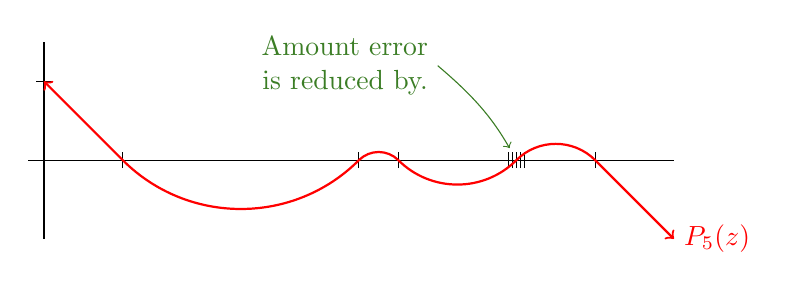
\begin{tikzpicture}[]

    \draw (0, -1) -- (0, 1.5);
    \draw (-0.2, 0) -- (8, 0);

    \foreach \x in {1, 4, 4.5, 6, 7}{
        \draw[xshift=\x cm] (0, -0.1) -- (0, 0.1) ;
    };

    \foreach \x in {5.9, 5.95, ..., 6.1}{
        \draw[xshift=\x cm] (0, -0.1) -- (0, 0.1) ;
    };

    \draw[yshift=1cm, rotate=90] (0, -0.1)  -- (0, 0.1) ;

    \draw[<->, red, thick]
    (0, 1) to
    (1, 0) to[bend right = 45]
    (4, 0) to[bend left = 45]
    (4.5, 0) to[bend right = 45]
    (6, 0) to[bend left = 45]
    (7, 0) to (8, -1) node[right]{$P_5(z)$}
    ;

    \draw[OliveGreen, shorten >=5pt, ->] (5, 1.2) node[left, text width = 3cm, align=right]{Amount error is reduced by.} to[bend left=10] (6, 0);

\end{tikzpicture}

\end{center}

In a general case where $A$ has a largest eigenvalue $\lambda_{\max}$ and a smallest eigenvalue $\lambda_{\min}$, and the other eigenvalues are more or less evenly distributed in $[\lambda_{\min}, \lambda_{\max}]$

\begin{equation*}
    \lvert\lvert \vec{e}^{\,(i)} \rvert\rvert_{A}
    \leq
    2
    \left(
    \frac{\sqrt{\kappa} - 1}{\sqrt{\kappa} + 1}
    \right)^i
    \lvert\lvert \vec{e}^{\,(0)} \rvert\rvert_{A}
\end{equation*}
where $\kappa = \lambda_{\max}/\lambda_{\min} = \sigma_{\max}/\sigma_{\min}$ is the condition number of $A$.

In many situations, the most expensive part of CG, or another Krylov solver, is the matvecs. However, once we've reduced this cost to $\bigO{n}$ operations, either because $A$ is sparse of hase structure (KIFMM), the bost of the matvec can not be reduced further with respect to complexity. Another way to further reduce the cost is to use a \underline{preconditioner}.

